L'équation de Nagumo (ou FitzHugh-Nagumo) est issue de modèles de transmission de l'information nerveuse \cite{FITZHUGH1961445}.
Nous utilisons la forme spatiale de l'équation \cite{keener1998mathematical} avec un terme de réaction cubique pour ajouter de la non-linéarité:
\begin{align}
    \dt{u} = \underbrace{D \dxx{u}}_{\text{diffusion}}
            - \underbrace{ku(1-u^2)}_{\text{réaction}}.
\end{align}
\paragraph{Solutions Analytiques}
Cette équation admet des solutions propagatives sous la forme:
\paragraph{Analyse Qualitative}
Le terme de diffusion est classique, il est non-local et une fois discrétisé à l'ordre deux ses valeurs propres associées sont 
$\{ ... \}$, ainsi la raideur croit linéairement avec le coefficient de diffusion $D$ et quadratiquement avec la finesse du maillage $\Delta x$.
En partant d'une solution initiale ..., 
la solution reste entre 0 et 1. Ainsi le terme de réaction est local, et ses valeurs propres sont comprises entre ...
En effet: 
\begin{align}
    R(u) = ku(1-u^2),\\
    R'(u) = k (1 - 3u^2).
\end{align}

\begin{figure}[htbp]
    \centering
    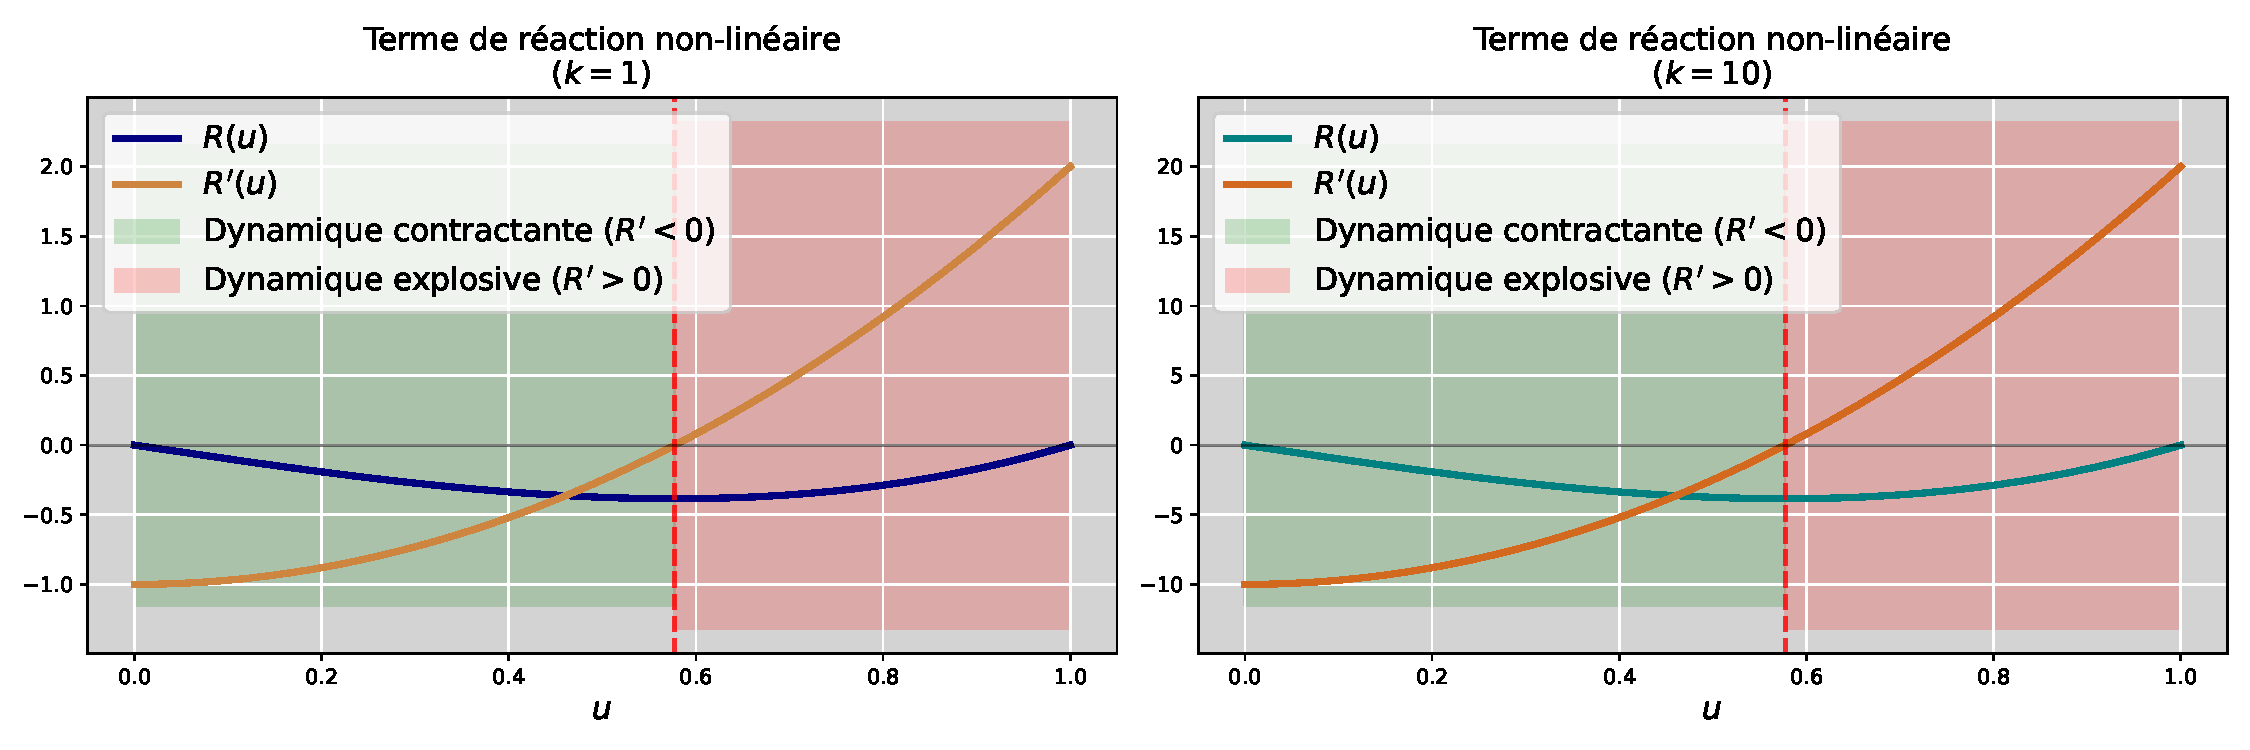
\includegraphics[width=\textwidth]{media/4_travail/2_nagumo/raideur_reaction_nagumo.pdf}
    \caption{Plage de valeurs du terme de réaction non-linéaire et de sa différentielle pour deux coefficients de réactions: $k=1$ et $k=10$.}
    \label{fig:raideur_reaction_nagumo}
\end{figure}